\documentclass{article}

\usepackage{filecontents}
\usepackage{tikz}
\usepackage{amsmath}
\usepackage{amsfonts}
\usepackage[bookmarks=true]{hyperref}
\input{util/util.tex}

\def\R{\ensuremath{\mathbb{R}}}
\begin{filecontents}{tmp.bib}
@book{boyd,
  title={\href{http://stanford.edu/~boyd/cvxbook/}{Convex Optimization}}, author={Boyd, Stephen and Vandenberghe, Lieven},
  year={2004},
  publisher={Cambridge university press}
}

\end{filecontents}

\begin{document} 

\title{Convexity Constraints in Optimization over Functional Spaces}
\author{Andreas Orthey}
\date{}
\maketitle

%%%%%%%%%%%%%%%%%
Let $\btau \in \F = C([0,1],X)$ with $\F$ being an infinite dimensional
functional space containing all continuous functions from $[0,1]$ to a space
$X$. We can represent $\F$ by an orthonormal basis of an infinite number of
basis functions $\{f_1,f_2,\cdots\}$. Any function $\btau$ in $\F$ can then be
written as a linear combination of basis functions as

\begin{equation}
        \begin{aligned}
                \btau(t) &= \sum\limits_{k=0}^\infty w_k f_k(t)
        \end{aligned}
\end{equation}

whereby $w_k$ are called the coefficients of the basis functions. Optimization
over $\F$ can now be done by optimizing over the linear coefficients $w_k$,
corresponding to a linear program.

\begin{equation}
        \begin{aligned}
                &\underset{\{w_1,w_2,\cdots\}}{\text{optimize }}&&
                \btau = \sum\limits_{k=0}^\infty w_k f_k(t)\\
                %&\text{subject to }&& a_i^T y + R\|a_i\|_2 \leq b_i\\
                %&&& R \geq 0
        \end{aligned}
\end{equation}

Let us approximate this linear program by using only a finite number of basis
function, corresponding to a subspace of $\F$. This corresponds to a loss of
completeness. However, since high frequency functions
are often undesirable in motion planning, this approximation will actually be
almost not noticeable. Let us choose a $K\gg0$ such that

\begin{equation}
        \begin{aligned}
                &\underset{\{w_1,\cdots,w_K\}}{\text{optimize }}&&
                \tau = \sum\limits_{k=0}^K w_k f_k(t)\\
                %&\text{subject to }&& a_i^T y + R\|a_i\|_2 \leq b_i\\
                %&&& R \geq 0
        \end{aligned}
\end{equation}

This convex (linear) program will be our (approximate) representation of the functional
space $\F$. 

\newpage
\section{Classical Convex Constraints}
We can now apply any convex constraints on the functional space, so
that we preserve convexity of our optimization procedure. A good overview is
given by \cite{boyd}. We will try to list here all known convex constraints, whereby
\begin{itemize}
        \item LEC = Linear Equality Constraint
        \item LIC = Linear Inequality Constraint
        \item QEC = Quadratic Equality Constraint
        \item QIC = Quadratic Inequality Constraint
        \item CEC = Convex Equality Constraint
        \item CIC = Convex Inequality Constraint
\end{itemize}

\subsection{Interpolation Condition (LEC)}
At point $t_i$, we like the function $\tau$ to have the value $z_i$,
corresponding for example to a waypoint at $z_i$. 
\begin{equation}
        \begin{aligned}
                \boxed{\tau(t_i) = z_i, \hspace{0.5cm}i=1,\cdots,m}
        \end{aligned}
\end{equation}
this is a LEC on the functional space.

\subsection{Neighborhood Constraint (LIC)}

We can also require the
function to be in an $\epsilon$-neighborhood of the waypoint at point $t_i$ as:
\begin{equation}
        \begin{aligned}
                \boxed{\|\tau(t_i) - z_i\|_2 \leq \eps \hspace{0.5cm}i=1,\cdots,m}
        \end{aligned}
\end{equation}

\subsection{Polytope Constraint (LIC)}
Going even further, we can restrict the position of $\tau$ at point $t_i$ to any
convex polytope $P=\{x| Ax\leq b\}$ as
\begin{equation}
        \begin{aligned}
                \boxed{A\tau(t_i) \leq b \hspace{0.5cm}i=1,\cdots,m}
        \end{aligned}
\end{equation}

\subsection{Lipschitz Constraint (LIC)}
\begin{equation}
        \begin{aligned}
                \boxed{\|\tau(t_j)-\tau(t_k)\| \leq L\|t_j-t_k\| \hspace{0.5cm}i=1,\cdots,m}
        \end{aligned}
\end{equation}

\newpage
\section{Convex Derivative Constraints}

Let us assume that $\F$ is actually $\C^1$, contains only functions which are
differentiable. Given a point $t_i$, the derivative of $\tau$ is given by

\begin{equation}
        \begin{aligned}
                \dfrac{d}{dt}\tau(t) = \sum\limits_{k=0}^K w_k \dfrac{d}{dt} f_k(t)
        \end{aligned}
\end{equation}
which is again a linear function of x. We can therefore apply any constraints
which we applied to $\tau$ also to its derivative $\dtau$.


\subsection{Maximum Gradient Norm (QIC)}
If we like to constraint the maximum gradient of $\tau$ (corresponding to a
maximum speed), we can do this via a QIC
\begin{equation}
        \begin{aligned}
                \boxed{\|\dtau(t_i)\| \leq M}
        \end{aligned}
\end{equation}

\subsection{Monotonity (LIC)}

If we like our function to be increasing we can restrict the derivative to the
positive halfspace
\begin{equation}
        \begin{aligned}
                \boxed{\tau(t_i) \geq 0 \hspace{0.5cm}i=1,\cdots,m}
        \end{aligned}
\end{equation}


\section{Combination Constraints}

\subsection{Circle on Polygonal Surface Constraint}

\begin{figure}[h]
\centering
\scalebox{0.6}{%\centering
%\scalebox{0.8}{
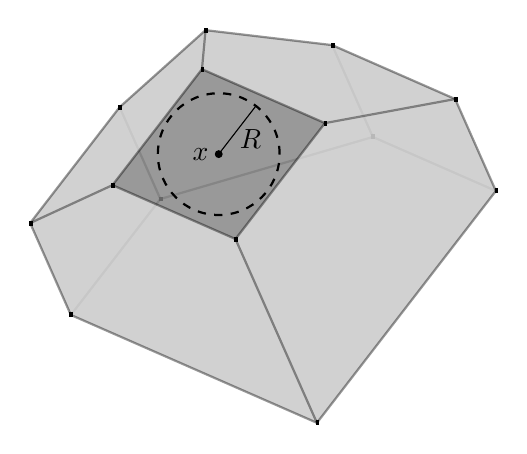
\begin{tikzpicture}
        [x={(0.258520cm, -0.583496cm)},
        y={(0.781193cm, -0.342529cm)},
        z={(-0.568247cm, -0.736347cm)},
        scale=2.000000,
        back/.style={loosely dotted, thin},
        edge/.style={color=black, thick, opacity=0.4},
        circle/.style={color=black, thick, dashed},
        facet/.style={fill=black!20,color=black!20,fill opacity=0.9},
        specialFacet/.style={fill=black!30,color=black!50,fill opacity=0.8},
        vertex/.style={inner sep=0.5pt,circle,draw=black!25!black,fill=black!75!black,thick,anchor=base},
        vertexC/.style={inner sep=5pt,circle,draw=black!100!black,fill=black!100!black,thick,anchor=base}]
%
%
%% Coordinate of the vertices:
%%

\coordinate (0.5, 0.5, -1.05) at (0.5, 0.5, 1.05);

\coordinate (-0.500, -0.500, -0.500) at (-0.500, -0.500, -0.500);
\coordinate (-1.00, 0.000, 0.000) at (-1.00, 0.000, 0.000);
\coordinate (-1.00, 0.000, 1.00) at (-1.00, 0.000, 1.00);
\coordinate (-1.00, 1.00, 0.000) at (-1.00, 1.00, 0.000);
\coordinate (-1.00, 1.00, 1.00) at (-1.00, 1.00, 1.00);
\coordinate (0.000, -1.00, 0.000) at (0.000, -1.00, 0.000);
\coordinate (0.000, -1.00, 1.00) at (0.000, -1.00, 1.00);
\coordinate (0.000, 0.000, -1.00) at (0.000, 0.000, -1.00);
\coordinate (0.000, 1.00, -1.00) at (0.000, 1.00, -1.00);
\coordinate (1.00, -1.00, 0.000) at (1.00, -1.00, 0.000);
\coordinate (1.00, -1.00, 1.00) at (1.00, -1.00, 1.00);
\coordinate (1.00, 0.000, -1.00) at (1.00, 0.000, -1.00);
\coordinate (1.00, 1.00, -1.00) at (1.00, 1.00, -1.00);
\coordinate (1.00, 1.00, 1.00) at (1.00, 1.00, 1.00);
%%
%%
%% Drawing edges in the back
%%
%%
%%
%% Drawing vertices in the back
%%
\node[vertex] at (1.00, -1.00, 0.000)     {};
\node[vertex] at (1.00, 0.000, -1.00)     {};
%%
%%
%% Drawing the facets
%%
\draw[edge] (0.000, -1.00, 0.000) -- (1.00, -1.00, 0.000);
\draw[edge] (0.000, 0.000, -1.00) -- (1.00, 0.000, -1.00);
\draw[edge] (1.00, 0.000, -1.00) -- (1.00, 1.00, -1.00);
\draw[edge] (1.00, -1.00, 0.000) -- (1.00, -1.00, 1.00);
\draw[edge] (1.00, -1.00, 0.000) -- (1.00, 0.000, -1.00);

\fill[facet] (1.00, 1.00, 1.00) -- (-1.00, 1.00, 1.00) -- (-1.00, 1.00, 0.000) -- (0.000, 1.00, -1.00) -- (1.00, 1.00, -1.00) -- cycle {};
\fill[facet] (1.00, 1.00, 1.00) -- (-1.00, 1.00, 1.00) -- (-1.00, 0.000, 1.00) -- (0.000, -1.00, 1.00) -- (1.00, -1.00, 1.00) -- cycle {};
\fill[facet] (0.000, -1.00, 1.00) -- (-1.00, 0.000, 1.00) -- (-1.00, 0.000, 0.000) -- (-0.500, -0.500, -0.500) -- (0.000, -1.00, 0.000) -- cycle {};
\fill[facet] (0.000, 1.00, -1.00) -- (-1.00, 1.00, 0.000) -- (-1.00, 0.000, 0.000) -- (-0.500, -0.500, -0.500) -- (0.000, 0.000, -1.00) -- cycle {};
\fill[specialFacet] (-1.00, 1.00, 1.00) -- (-1.00, 0.000, 1.00) -- (-1.00, 0.000, 0.000) -- (-1.00, 1.00, 0.000) -- cycle {};
\draw[edge] (1.00, -1.00, 1.00) -- (1.00, 1.00, 1.00);
\draw[edge] (1.00, 1.00, -1.00) -- (1.00, 1.00, 1.00);
\draw[edge] (0.000, -1.00, 1.00) -- (1.00, -1.00, 1.00);
\draw[edge] (0.000, 0.000, -1.00) -- (0.000, 1.00, -1.00);
\draw[edge] (0.000, 1.00, -1.00) -- (1.00, 1.00, -1.00);
%%
%%
%% Drawing edges in the front
%%
\draw[edge] (-0.500, -0.500, -0.500) -- (-1.00, 0.000, 0.000);
\draw[edge] (-0.500, -0.500, -0.500) -- (0.000, -1.00, 0.000);
\draw[edge] (-0.500, -0.500, -0.500) -- (0.000, 0.000, -1.00);
\draw[edge] (-1.00, 0.000, 0.000) -- (-1.00, 0.000, 1.00);
\draw[edge] (-1.00, 0.000, 0.000) -- (-1.00, 1.00, 0.000);
\draw[edge] (-1.00, 0.000, 1.00) -- (-1.00, 1.00, 1.00);
\draw[edge] (-1.00, 0.000, 1.00) -- (0.000, -1.00, 1.00);
\draw[edge] (-1.00, 1.00, 0.000) -- (-1.00, 1.00, 1.00);
\draw[edge] (-1.00, 1.00, 0.000) -- (0.000, 1.00, -1.00);
\draw[edge] (-1.00, 1.00, 1.00) -- (1.00, 1.00, 1.00);
\draw[edge] (0.000, -1.00, 0.000) -- (0.000, -1.00, 1.00);
%%
%%
%% Drawing the vertices in the front
%%
\node[vertex] at (-0.500, -0.500, -0.500)     {};
\node[vertex] at (-1.00, 0.000, 0.000)     {};
\node[vertex] at (-1.00, 0.000, 1.00)     {};
\node[vertex] at (-1.00, 1.00, 0.000)     {};
\node[vertex] at (-1.00, 1.00, 1.00)     {};
\node[vertex] at (0.000, -1.00, 0.000)     {};
\node[vertex] at (0.000, -1.00, 1.00)     {};
\node[vertex] at (0.000, 0.000, -1.00)     {};
\node[vertex] at (0.000, 1.00, -1.00)     {};
\node[vertex] at (1.00, -1.00, 1.00)     {};
\node[vertex] at (1.00, 1.00, -1.00)     {};
\node[vertex] at (1.00, 1.00, 1.00)     {};
%%

\draw[fill=black,color=black] (-1.00, 0.500, 0.50) -- (-1.0,0.5,0.08) node[pos=0.3,right]{$R$};
\draw[thick,fill=black,color=black] (-1.00, 0.500, 0.500) circle (0.5pt) node[left] {$x$};
\draw[circle] (-1.00, 0.50, 0.50) circle (11pt);

\end{tikzpicture}
%}
%\caption{A polytope in $\R^3$ (light gray) and a surface element (dark gray)}
%\end{figure}

}
\end{figure}

Let a polytope be given by $P =\{x\in R^n|a_k x \leq b_k, k=1,\cdots,D\}$,
non-empty, bounded. Given a surface $p$ of this polytope, we can construct a
convex equation to determine if a point on the surface $p$ has a circle of radius $R$, which is fully contained in the surface element $p$. 

\begin{equation}
        \begin{aligned}
                        a_k^T x + R a_k^T a_k'&\leq b_k,&&\scalebox{0.9}{$i=\{1,\cdots,p-1,p+1,\cdots,T\}$}\\
                        a_p^Tx &= b_p\\
        \end{aligned}
\end{equation}
        whereby $R$ is the radius of the circle, $x$ the center, $a_p$ is the surface normal of the element $p$, and $a_k'$ is the
        orthogonal projection onto the hyperplane of $a_p$, i.e. $a_k' = a_k -
        (a_k^Ta_p)a_p$. %Visualized in Fig. \ref{fig:circleonsurface}. 
        This could correspond to the (circular) foot of a humanoid robot stepping on a box or another surface element. If our trajectory is actually a trajectory for a foot, we might want to restrict the whole foot to this surface element. The corresponding constraint on our trajectory would be


\begin{equation}
        \begin{aligned}
        \boxed{A \tau(t_i) \leq b - \eps \diag (A^T A')}
        \end{aligned}
\end{equation}
whereby we have $A=\{a_1,\cdots,a_D\}$ and $A'=\{a'_1,\cdots,a'_D\}$ with $a'_k = a_k - (a_k^Ta_p)a_p$











\bibliographystyle{plainnat}
\bibliography{tmp} 
\end{document}

